% Created 2023-03-17 Fri 20:39
% Intended LaTeX compiler: pdflatex
\documentclass[11pt]{article}
\usepackage[utf8]{inputenc}
\usepackage[T1]{fontenc}
\usepackage{graphicx}
\usepackage{longtable}
\usepackage{wrapfig}
\usepackage{rotating}
\usepackage[normalem]{ulem}
\usepackage{amsmath}
\usepackage{amssymb}
\usepackage{capt-of}
\usepackage{hyperref}
\usepackage{fancyhdr}
\usepackage[a4paper, total={6in, 8in}]{geometry}
\usepackage{fontspec}
\usepackage{amsmath}
\pagestyle{fancy}
\fancyhf{}
\lhead{190014935}
\rhead{CS4303 Practical 2 - 17/03/2023}
\fancyfoot[RO, LE] {Page \thepage}
\author{190014935}
\date{\today}
\title{CS4303 Practical 2 Report}
\hypersetup{
 pdfauthor={190014935},
 pdftitle={CS4303 Practical 2 Report},
 pdfkeywords={},
 pdfsubject={},
 pdfcreator={Emacs 27.2 (Org mode 9.6)}, 
 pdflang={English}}
\begin{document}

\maketitle
\tableofcontents


\section{Introduction}
\label{sec:org3934cb5}
For this practical, we were tasked with implementing a rogue-like game, where a player advances through procedurally
generated dungeons, and defeats enemies until its death. The goal of this practical overall is to understand and be
able to implement procedural level generation and AI into a game.

Overall, I have fully built a game which implements A* algorithm based AI and rudimentary behaviour, along with an
advanced rendering system.

\section{The Game}
\label{sec:orgd6d7351}
The implemented game closely resembles a classic rogue-like RPG-style game, and heavily references older raycaster-based
games, and the game \texttt{Wolfenstein 3D} in particular.

\subsection{Environment}
\label{sec:org01429bd}
The environment is a large maze-like level, from which the player traverses through. Each level is generated using
a binary space partitioning algorithm, which partitions a grid into a tree of rooms, which are then linked together
by simply tracing lines between them.

Better corridor tracing algorithms that perfectly trace corridors between rooms without intersecting with other rooms exist,
but the effect of having corridors going through other rooms inadvertedly gives interesting room patterns.

Rendering-wise, the map is visualized using a raycaster with rays traced in all 3 space axis,
with ceiling-size set as 3. This visualisation gives a sense of size to the rooms or corridors,
while making the player feel small.

\subsection{Player}
\label{sec:org073e6e0}
The player in this game is represented in first-person view with the raycaster. The user controls the player via basic
first-person controls (mouse, WASD keys). The first-person view and control have a very familiar and more personal effect
compared to top-down WASD only control and view - the user feels naturally more ``in the skin'' of the player with this
technique, which enhances tension during gameplay, and even allows for some occasional jumpscares.

\subsection{Enemies}
\label{sec:orga6e1054}
Enemies in this game are represented as orbs that usually follow an idle path until they become hostile.
Upon seeing the player, they immediately switch to a hostile state, in which they follow the player until either they lose
track of them, or reach them.

During battles, the orbs do not have many options and so the only thing they can do is attack. Albeit being a simple
battle behaviour, this system already makes the game interesting. The complexity of the battle mechanic comes instead from
user resource-management and player decision.

Another area of player decision regarding enemies lies in the player trying to remain as stealthy as possible as so not
to aggro the orbs. A more stealth or avoidance focused gameplay opens more gameplay opportunities for the player by trying
to go as far in the game as possible while battling as least as possible.

Finally, this game is supposed to be hard. Therefore, enemies are placed in each rooms except the starting one. This further
complexifies stealth-based gameplay as the player must make decisions on every room instead of casually wandering around.

\subsection{Items}
\label{sec:org4ac89bb}
There are 5 kinds of items a player can find in the wild -
\begin{itemize}
\item Potions/consumables - items that resplenish player health in a pinch,
\item Weapons - Allow the player to deal more damage during battle,
\item Armor - Allow the player to defend itself - and afflict the enemy with some affects upon successfully defending
against an attack, such as poison or strength attribute decrease.
\item Miscallaneous - Items with no purpose, which add to the final score at the end of the game.
\end{itemize}

Those items define player decision during gameplay. Gameplay-wise, only consumables can be used during and only during
explorations. They cannot be used during battles. This decision forces the player to think about its health between
fights and punishes players who do not do so.

Finally, instead of using a mana-focused system, armors have side effects imbued. The reasoning behind it is to do a more
grounded system, where magic is a rarity instead of a commodity. It also means that if a player relies on armor magic to do damage, then that is option is viable for gameplay.

The inventory is quite large, such that the player can get a big collection of items to choose from. The inventory is
accessible via the inventory page, and is fully operable by using the WASD keys to move around and the E key to select
and move items.

\subsection{Attributes}
\label{sec:orgb6b545d}
The entity attributes system is consisted of 6 attributes:
\begin{itemize}
\item Strength - determines how much a player deals damage at each battle round,
\item Endurance - determines player max health. It is important to keep that attribute high to get a good scaling health
against stronger enemies.
\item Dexterity - determinies player speed - that is whether the player will move first or last during an encounter. It
is important to keep that attribute high as a low dexterity means the player will most of the time move last against
other enemies, losing health on each encounter.
\item Luck - determines the item drops at each new level. It is the least important attribute, but a high luck attribute
increases chances a player will get new items.
\end{itemize}

At each level, an extra point is allocated to the player's attributes.
Such an attribute system means that player decision will be important during gameplay as
build viability will determine the likeliness that the player will be able to reach higher floors.

\subsection{Combat}
\label{sec:org08e1e92}
The combat system is a one-vs-one, Player-vs-Enemy system in which the player can choose between 3 different actions:
\begin{itemize}
\item Attack - direct attack on the enemy using the weapon at hand, or nothing if the player has no weapon in hand,
\item Defend - the player defends against the enemy - this uses the defense effect of the armor the player is usign.
\item Flee - flee the battle - the enemy may however become stronger next time.
\end{itemize}

The combat system is completely deterministic, such that the player can make more strategic decisions about the fights they
will take before engaging. Randomness comes from what attributes the enemies have, as enemies also gain attribute points
as well after each floor (1 attribute point per floor).

This simple battle system heavily depends on the attributes and the items the player has equipped. Therefore the best
determinant of player success will be the decisions they have made before a fight, and how they use their build to
their advantage during battle.

\subsection{Score}
\label{sec:orgce7d897}
The final score is a combination of multiple factors:
\begin{itemize}
\item The score of all the miscallaneous items in the inventory,
\item The number of enemies killed by the player - in terms of enemy XP, such that the score scales by enemy difficulty,
\item The floor reached - the most important score trait and the one with the most weight on the final score.
\end{itemize}

This score encourages the player to play in a style that favours going to higher floors, but still allows players to play
in whichever way they want.

\subsection{Game Menu and Help}
\label{sec:org07c6afa}
The game menu in this game is simple - it introduces the player to the game with a title drop and a binary choice -
to play the game, or to quit the game. The player jumps back to this menu after defeat as well.

Game instructions for the game are included in the \texttt{README.md} page, and describes the keybindings for all actions,
and how to play the game. Given more time, a help page would have been implemented, but this method is a faithful reminder
of how retro games used to insert all the game guidelines in the game notice.

\section{Design}
\label{sec:orgba79da2}

\subsection{Procedural Content Generation}
\label{sec:org5b02af1}
Each level in the game is procedurally generated. The process to generate is done sequentially in these steps:
\begin{itemize}
\item Using Binary Space Partitioning, divide spaces by 2 until it is determined that it is too small to divide further,
or it hits minimum room size, or the algorithm decides that this space is good enough for a room.
\item From the binary space partitioning nodes, rooms are constructed, with a size that is bound within the size of the partition.
The algorithm determines the size of the room as minimum half the size of the partition, and maximum the size of the
partition minus 1 cell on all sides of the room. This minimum offset for room size against partition size avoids having
rooms fused between themselves.
\item Corridors are traced between nearest rooms. The nearest room is determined by tracing between leaf nodes only if possible,
that is looking for the left-most node on the right side, and the right most node on the left side before tracing corridors. This technique avoids tracing corridors that go between too many rooms while still leaving some exceptions. This
small leeway for mistake allows for more paths, more spaciousness between rooms, while still keeping maze features such as
long dead ends and the such.
\item The player's starting position is determined as a random room in the map - this behaviour is fine and enemies
will not spawn in that room - to make sure that the player has some time to breath upon arriving to a new floor.
\item A portal room is determined and a portal is placed on a random location in that room. This determined where the player
must reach in order to go to the next floor. The portal room can end up in the starting room as well - this behaviour
is allowed as it is an easy way to let the player breath a bit more, and adds a bit of luck element to it.
\item Items are randomly generated accross rooms, with object rarity depending on the player's luck attribute. This means the
player will require to level up their luck attribute in order to get better loot.
\end{itemize}

Finally, all those steps use the same random object, initialized to the same seed. Therefore, levels are identically
reproducible using the right seed. This easens the debugging process during development, and with more time, would allow
to redo certain levels if the right floor number and seed is known by the user.
\subsection{Artificial Intelligence}
\label{sec:org4612bd6}

The artificial intelligence in this game uses a combination of a simple decision tree and A* search to give
a satisfying feeling to the orbs that charge towards the player.

The decision tree for the AI does in total 3 checks to determinie behaviour:
\begin{itemize}
\item The AI sees the player:
\begin{itemize}
\item Become hostile
\end{itemize}
\item If the AI is hostile:
\begin{itemize}
\item If it sees the player, go towards the player (Use A*),
\item If it doesn't see the player, go to the last known location of the player (Use previously registered A* path),
\end{itemize}
\item If the AI is idle:
\begin{itemize}
\item Move between 2 locations in the same room - going left and right or up and down a room to survey the area.
\end{itemize}
\end{itemize}

AI vision of the player is determined by casting a ray from the enemy to the player. If the ray hits a wall before
hitting the player, or the length of the ray is too long, then it is determined that the enemy does not see the player.

Finally, the A* algorithm keeps track of the previously found path. While this may enquire if the target's position changes
that the path may not be the most optimal, it optimises calculation time for the next time the A* algorithm is called.

\subsection{Raycasting Renderer}
\label{sec:orgc2ced6c}


The main feature of this game is how the whole map and all the sprites are visualised using raycasting.
Raycasting is a rendering technique that was previously done in older games to cheaply render an environment in a 3D-like
manner. However, raycasting is done in 2D worlds, hence the term of ``fake 3D''.

The most famous example of a game using raycasting is ``Wolfenstein 3D'', released in 1992 by id Software. At the time, this
game was considered a graphical novelty as the raycasting technique allowed the game to be run on virtually any computer
in that era. This game is also today considered one of the founders and grandpa of the First Person Shooter genre, with
the try father of First Person Shooter games being Doom, a game made 2 years later by the same group, using a much more
advanced but still extremely efficient game renderer, using Binary Space Partitioning to render the game geometry.

\subsubsection{Raycasting Technique}
\label{sec:org914b1bb}

Here, the technique used to the render the area is raycasting done using GPU acceleration: basically, the raycaster is
implemented here as a fragment shader, where each pixel is a ray traced in a certain direction determined by a plane,
accross the x, y and z value.

Usually, raycasting is done on the CPU, and uses only the x and y axis, is run on the width of the screen, and determines
line height on ray distance. Here, thanks to the power of the fragment shader. A ray can be traced on both the x, y and
z axis, allowing for an effectively more 3D-looking render visual. Furthermore, per-pixel depth is then calculated
and added to the GPU's depth buffer, which helps for sprite rendering later on.

The advantage of doing the raycasting as a fragment shader is 3-fold:
\begin{enumerate}
\item GPUs are extremely fast at parallelization and raycasting is extremely parallelizable. Therefore, instead of sequentially
tracing rays on the CPU, all rays are calculated at once on the GPU.
\item Usual GPU raycasting determines perspective from the rays. Here, the only thing the shader needs to do is get the color
of the thing is has hit and display it on its own pixel. Giving a better effect for effectively less calculation.
\item It is easy after casting the ray to determine at which exact location it hit a wall or a ceiling. From this, texture
coordinates can be calculated. Therefore, textured GPU raycasting becomes far easier than its CPU counterpart.
\end{enumerate}

Finally, the main point of raycasting here, and why it was extremely efficient in Wolfenstein 3D, was how it takes
advantage of the grid nature of the map to efficiently and accurately calculate the position of each pixels.
Indeed, the raycasting algorithm here takes the whole level as a texture image to the fragment shader. Then, during ray
calculation, instead of adding increments at each step of the ray, it is possible to determine the next position at
which the ray will hit a new grid of the cell. This technique is far more efficient and far more accurate than simple
step increases, using max 20 steps to render walls that are far away, instead of using far more small value iterations.

\subsubsection{Sprite Rendering}
\label{sec:org8cc00fa}

Finally, sprites are rendered on a classic 3D perspective object-based rendering basis. Thanks to the depth buffer saved
from the raycasting, depth can be determined with each sprite on their fragment shader. GPU depth testing will finally
determine what fragment is on top and display the pixel. This method allows all sprites to be rendered correctly, to
be hidden when they are supposed to be hidden, and shown when the player can immediately look at them.

As there aren't too many sprites in a level, and they're basically all rectangles, it is efficient to do object-based
rendering for them. Meanwhile, this is not done for the map as that would mean using cubes for each square of the map.

Given more time, more of the vertex calculations for sprites could be done on the GPU, but processing does not play nicely
with custom shaders and the 3D renderer.

Therefore, the current rendering system is both efficient and great looking, giving the game the look that it has.

\section{Conclusion}
\label{sec:org2792ad3}
Overall, I have managed to fulfill all the requirements of the practical and more, with a gameplay-efficient AI, satisfying
terrain generation, and a very entertaining rendering style.

Raycasting is a classic rendering style which I love, and this game pays hommage to older games and
the first person genre in an playful way.

Given more time, I would have included more AI options and gameplay features, along with more options in the raycaster, such
as variable room ceiling sizes.

\section{Pictures}
\label{sec:orgb28ba4b}
\begin{figure}[htbp]
\centering
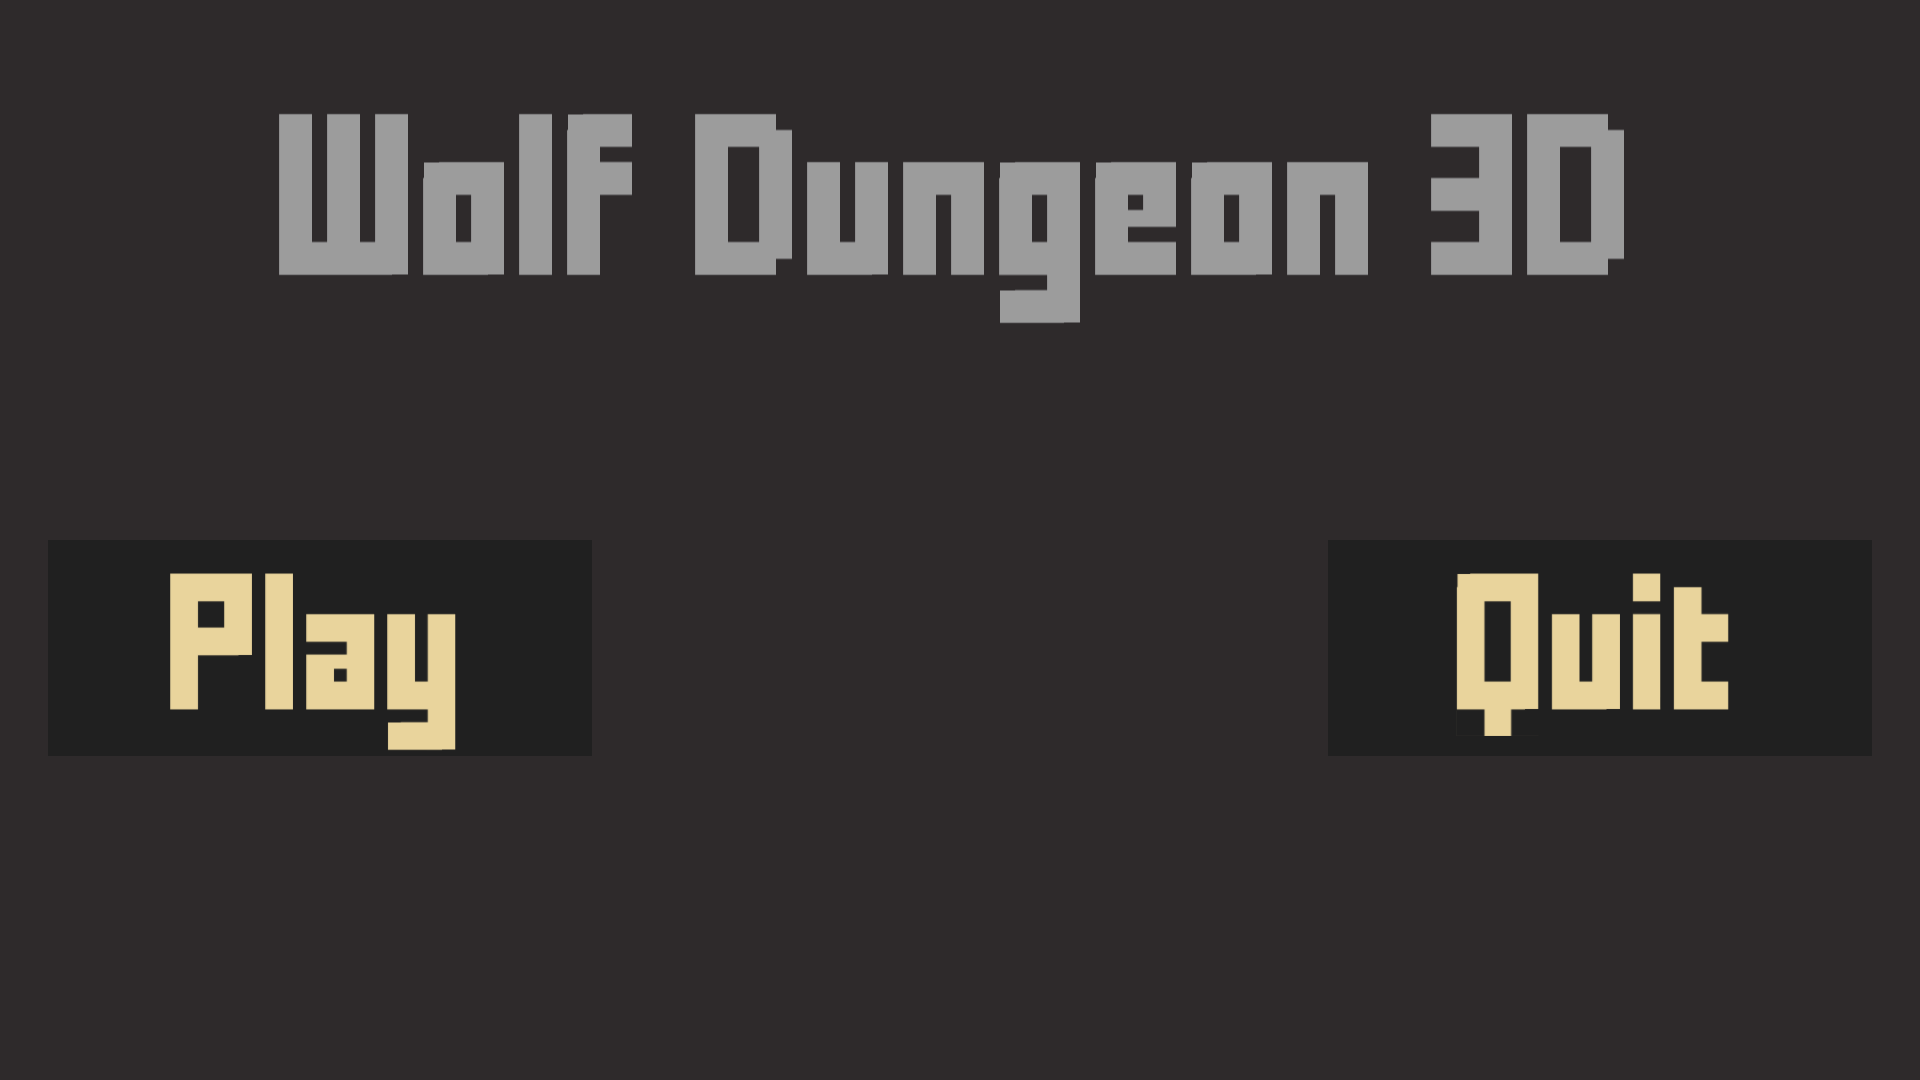
\includegraphics[width=.9\linewidth]{./mainMenu.png}
\caption{Main Menu}
\end{figure}

\begin{figure}[htbp]
\centering
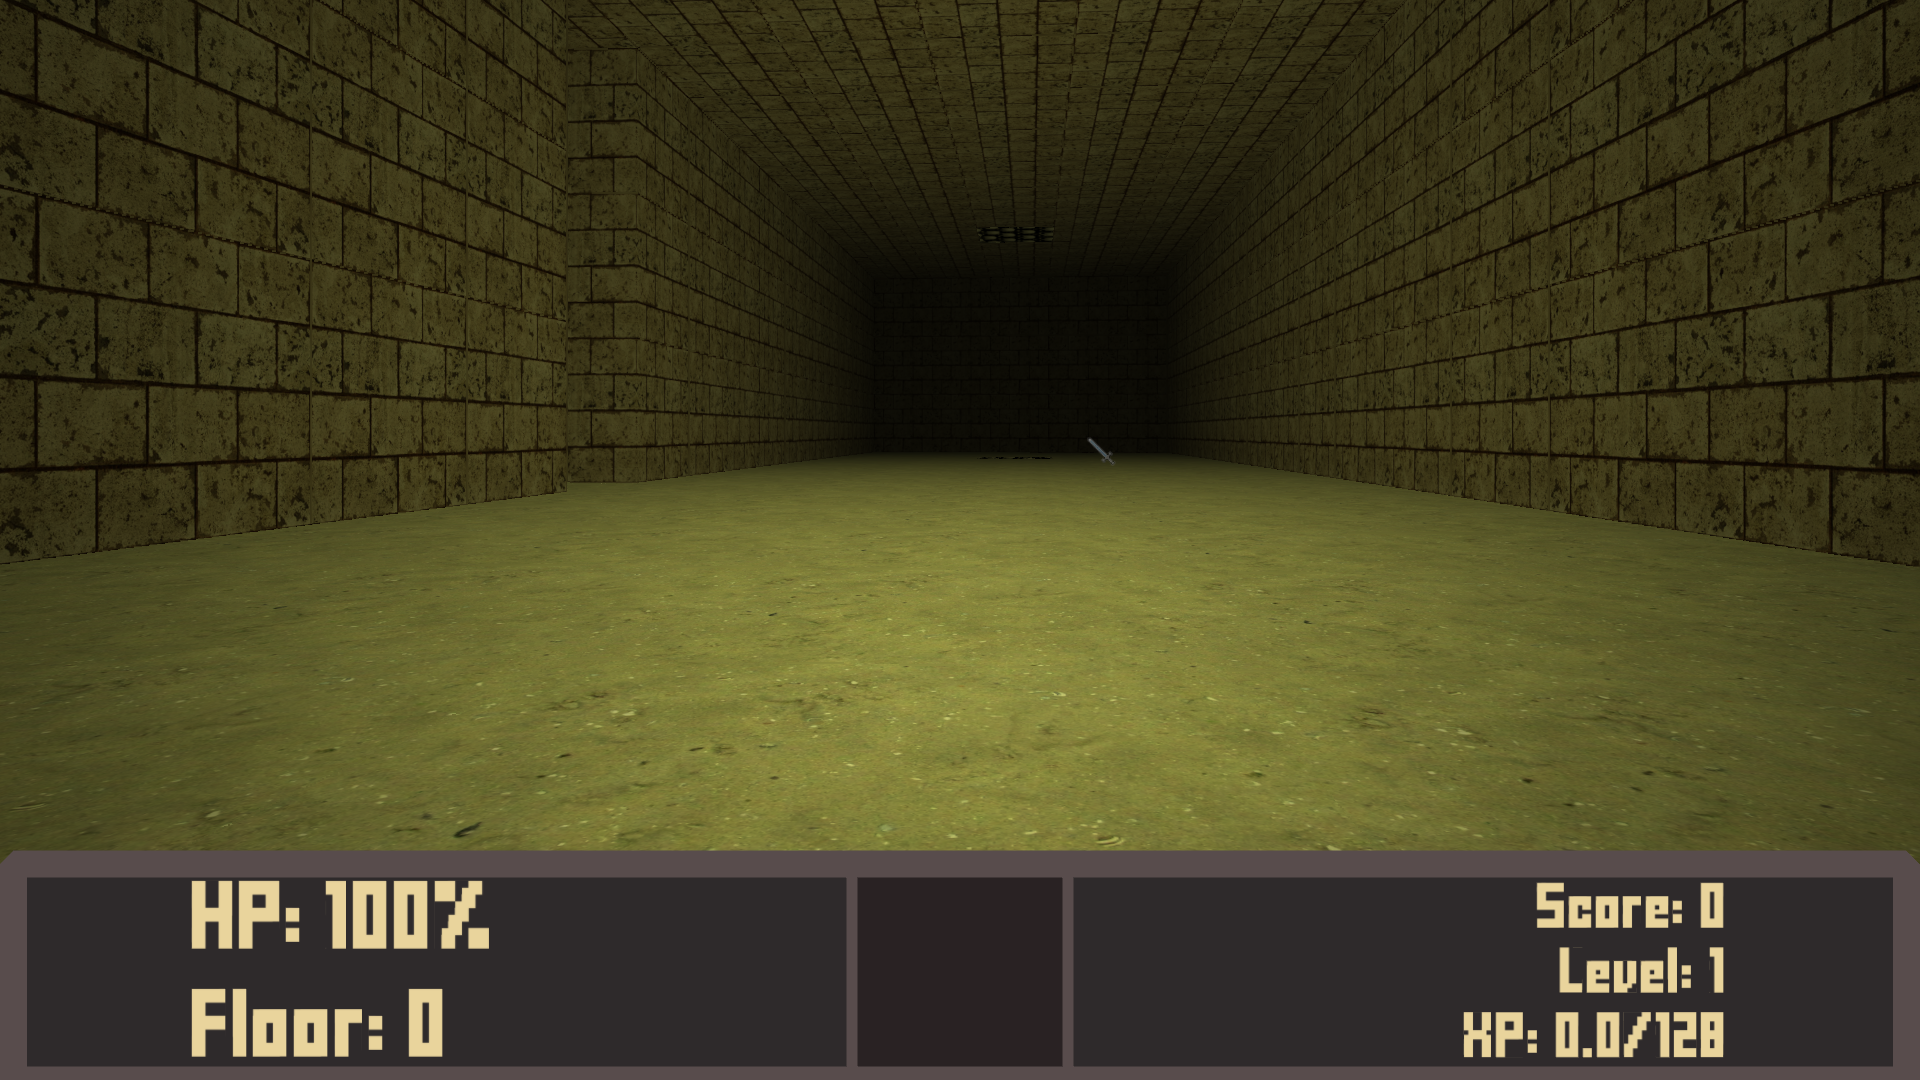
\includegraphics[width=.9\linewidth]{./mainGame.png}
\caption{Main Game Screen}
\end{figure}

\begin{figure}[htbp]
\centering
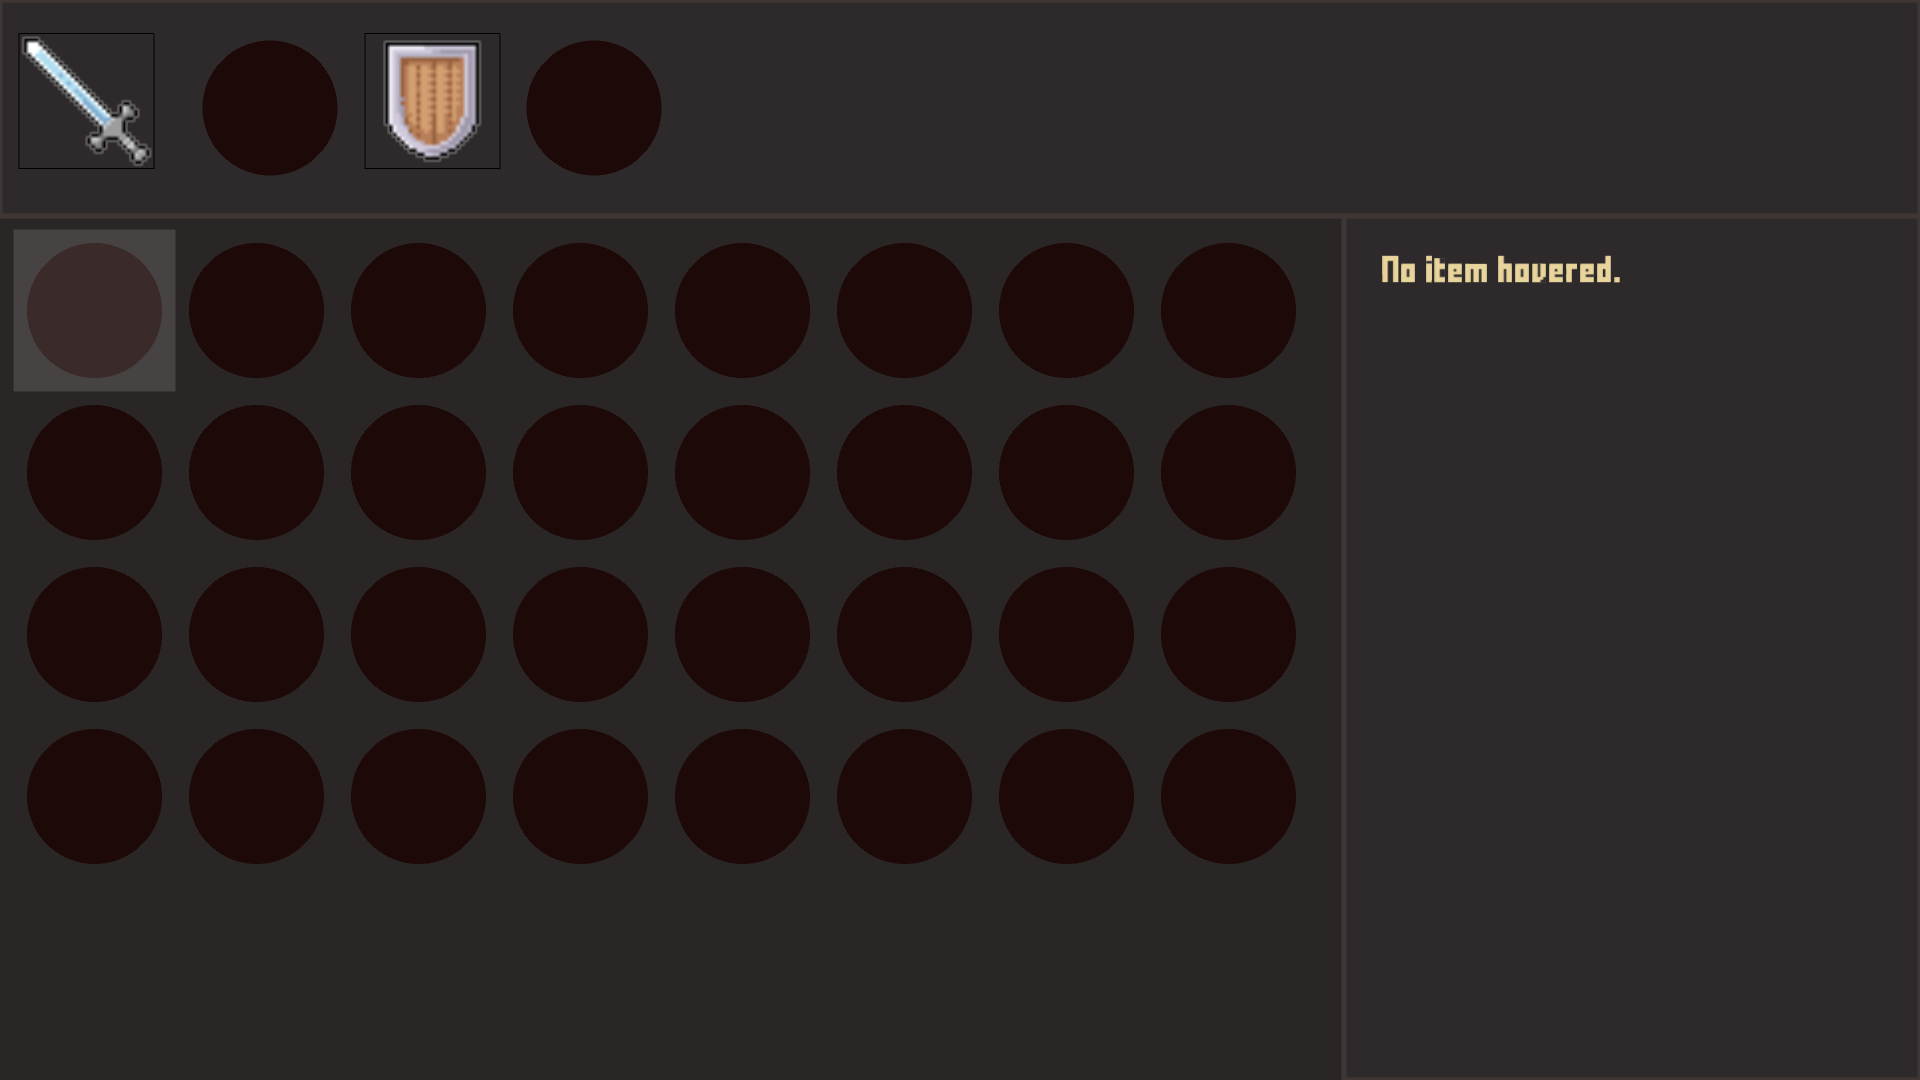
\includegraphics[width=.9\linewidth]{./inventory.png}
\caption{Inventory}
\end{figure}

\begin{figure}[htbp]
\centering
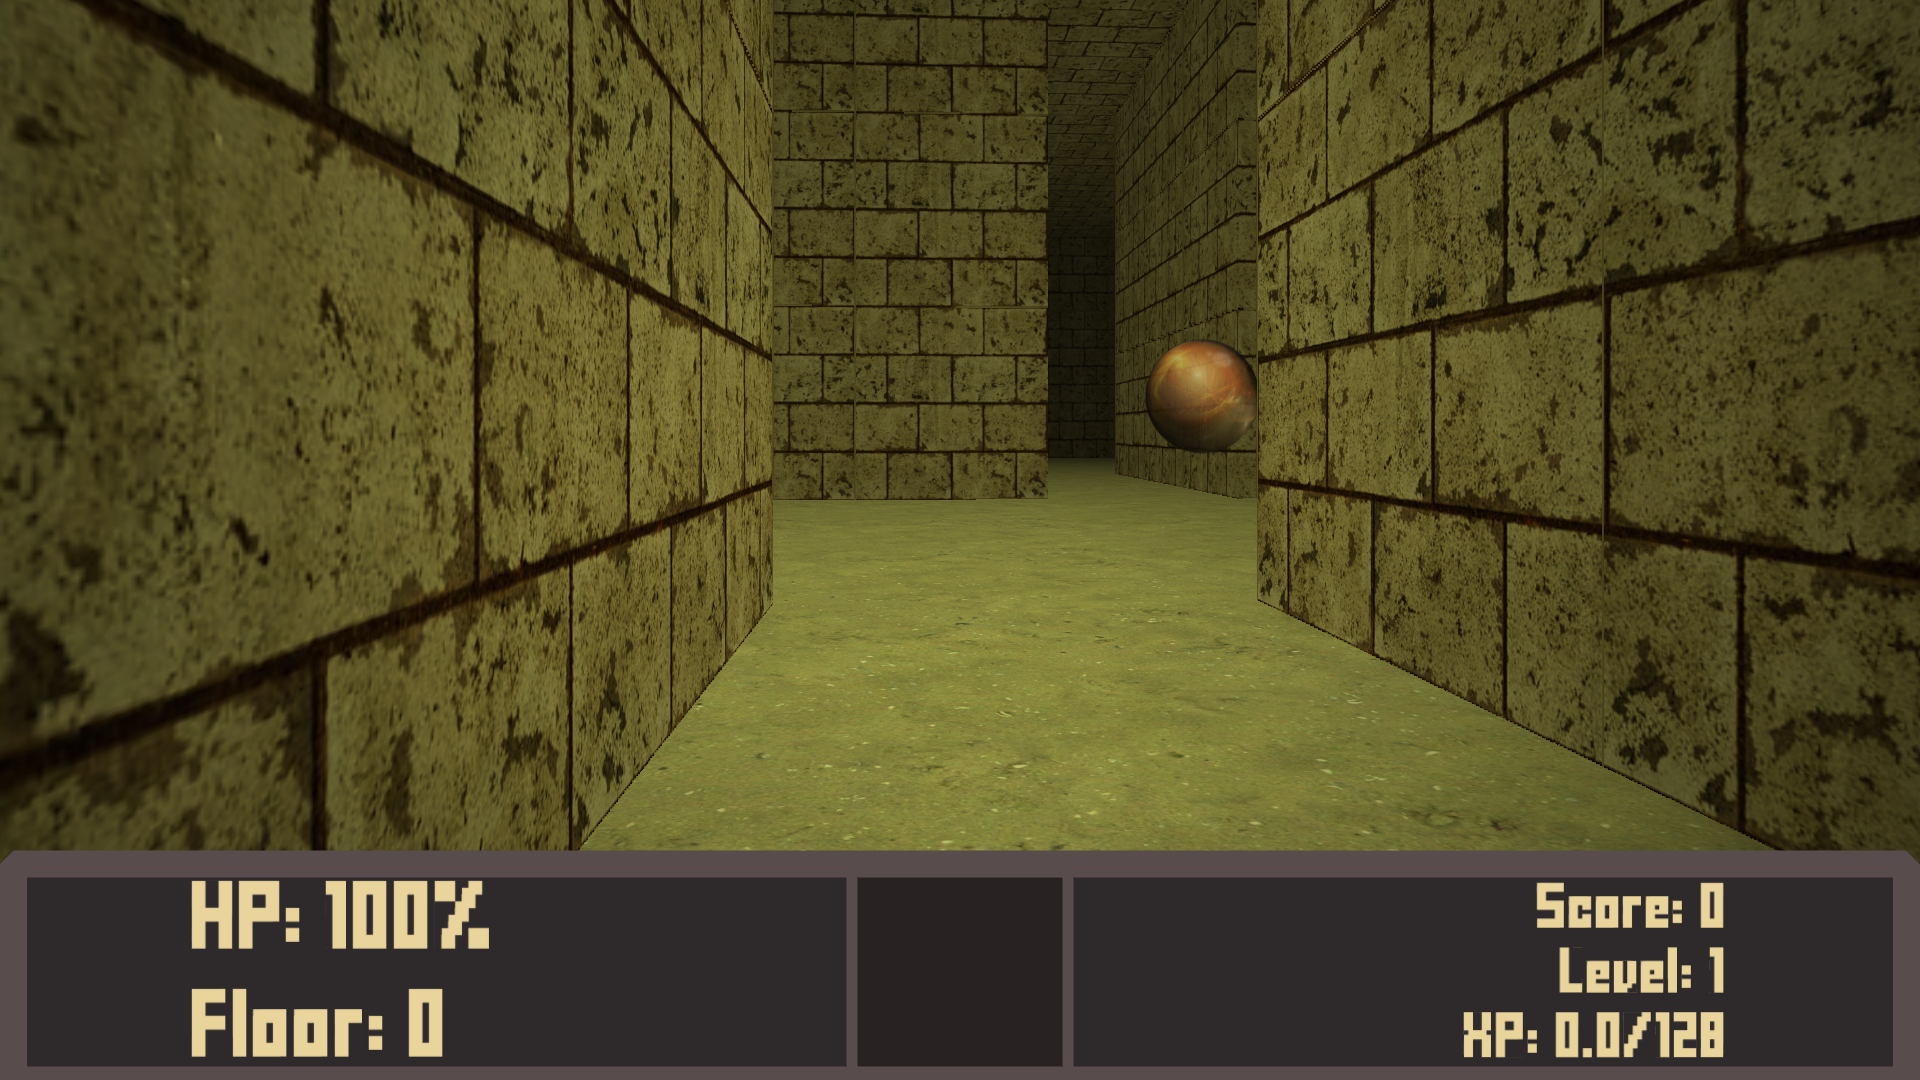
\includegraphics[width=.9\linewidth]{./enemy.png}
\caption{Enemy in the distance}
\end{figure}

\begin{figure}[htbp]
\centering
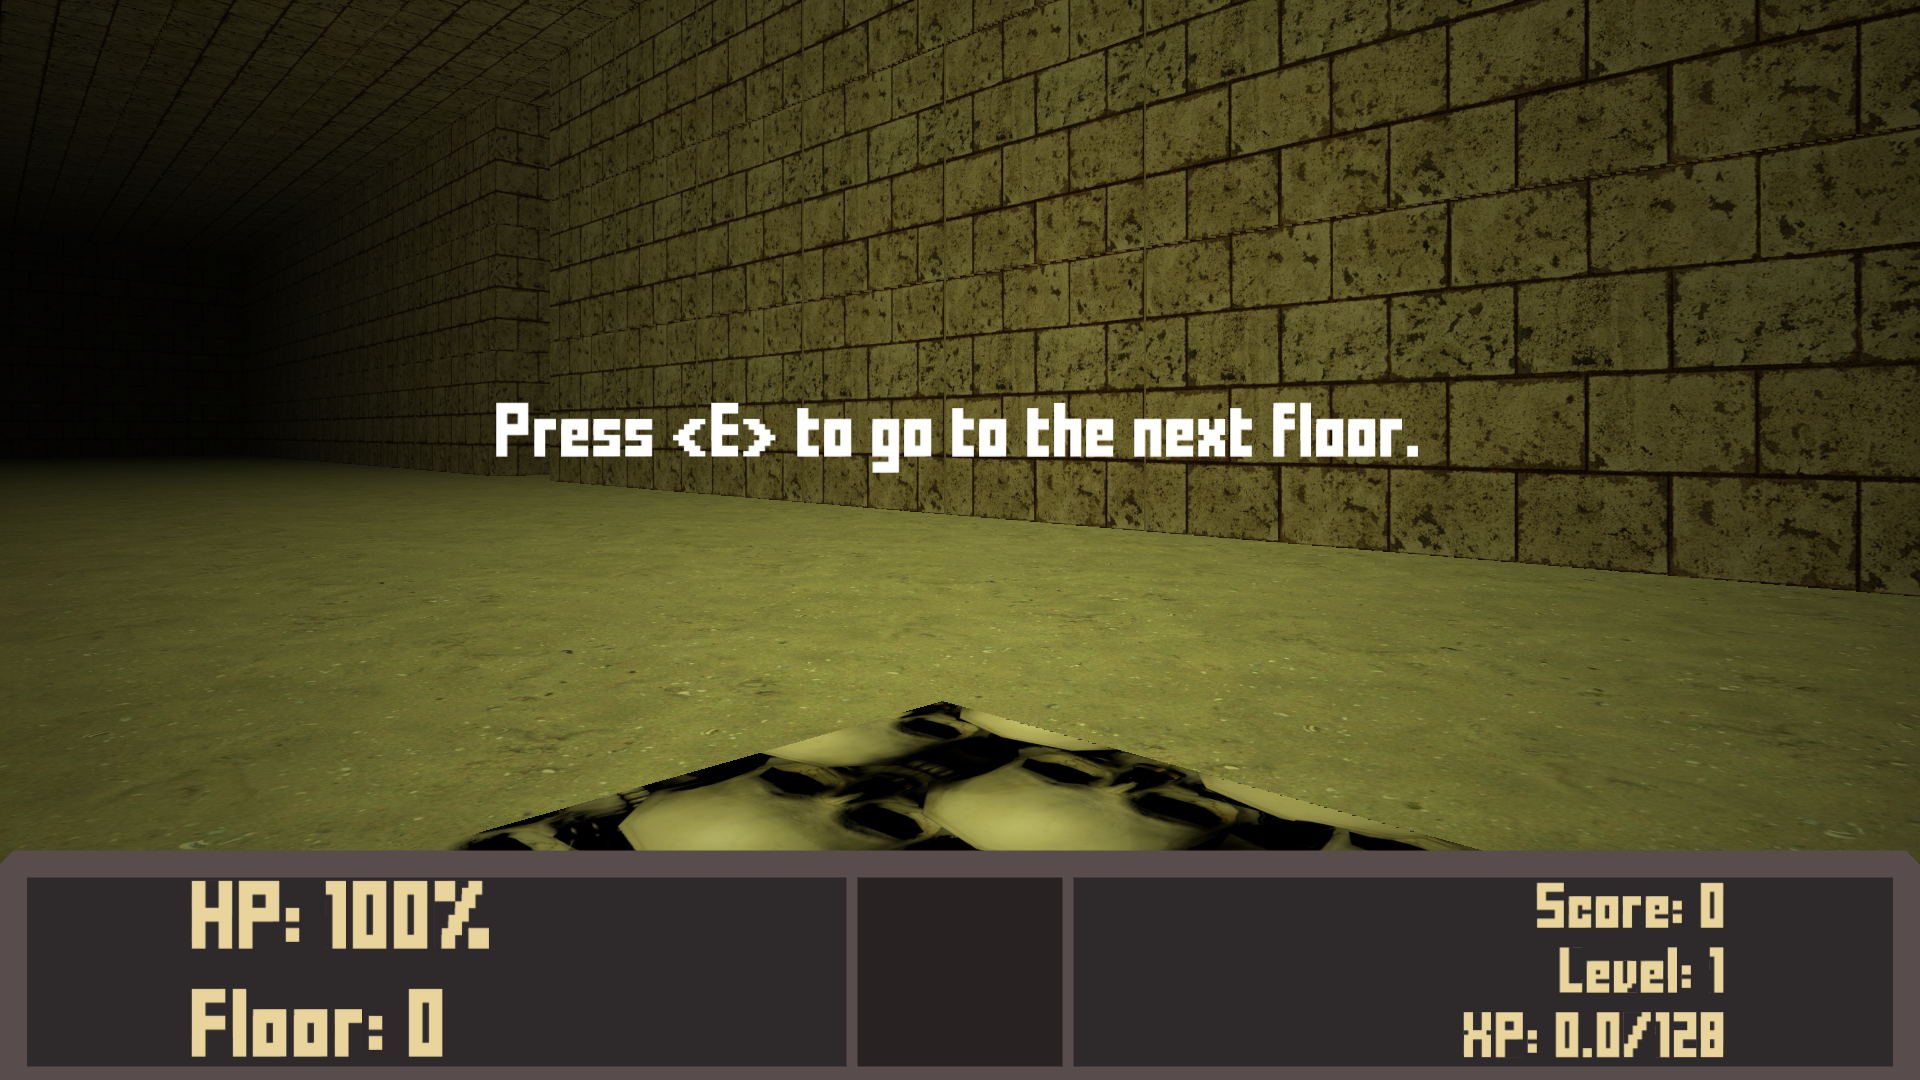
\includegraphics[width=.9\linewidth]{./portal.png}
\caption{Exit portal}
\end{figure}

\begin{figure}[htbp]
\centering
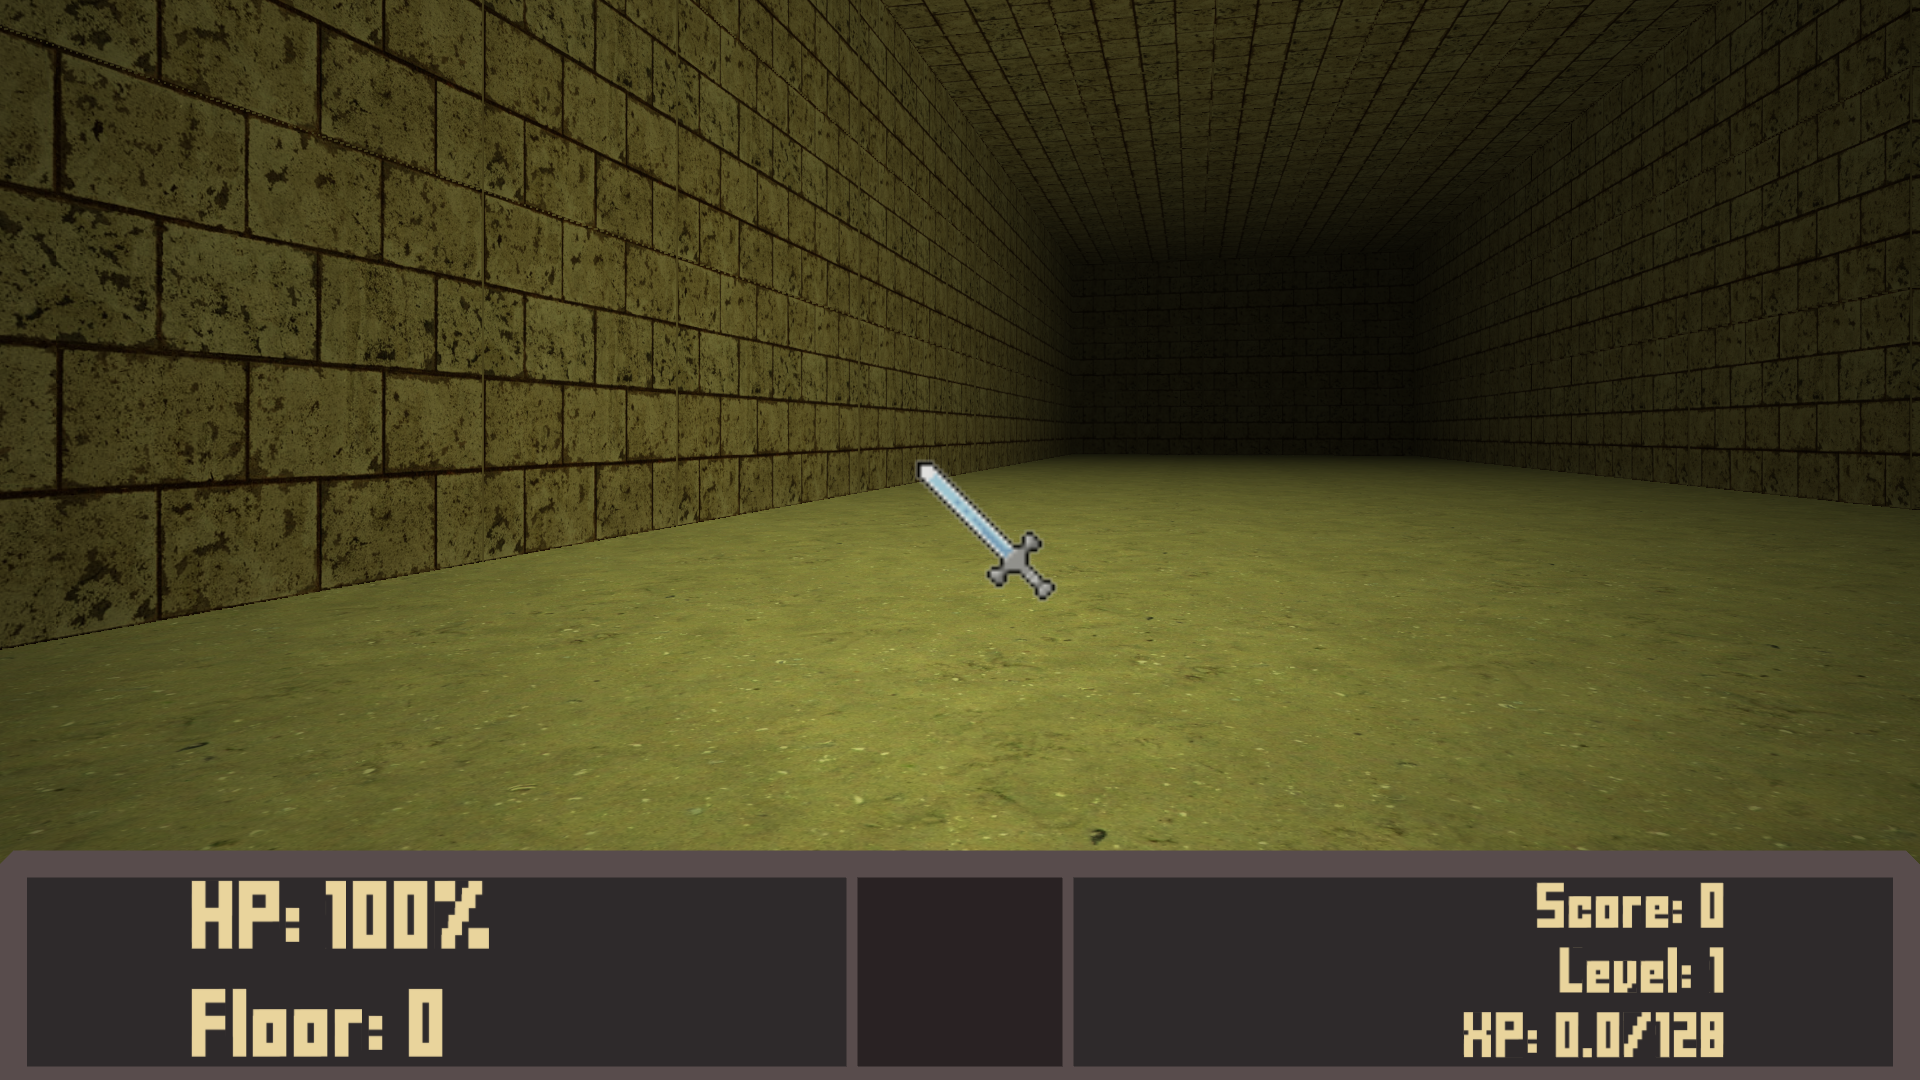
\includegraphics[width=.9\linewidth]{./weapon_item.png}
\caption{Grabbable weapon item}
\end{figure}
\begin{figure}[htbp]
\centering
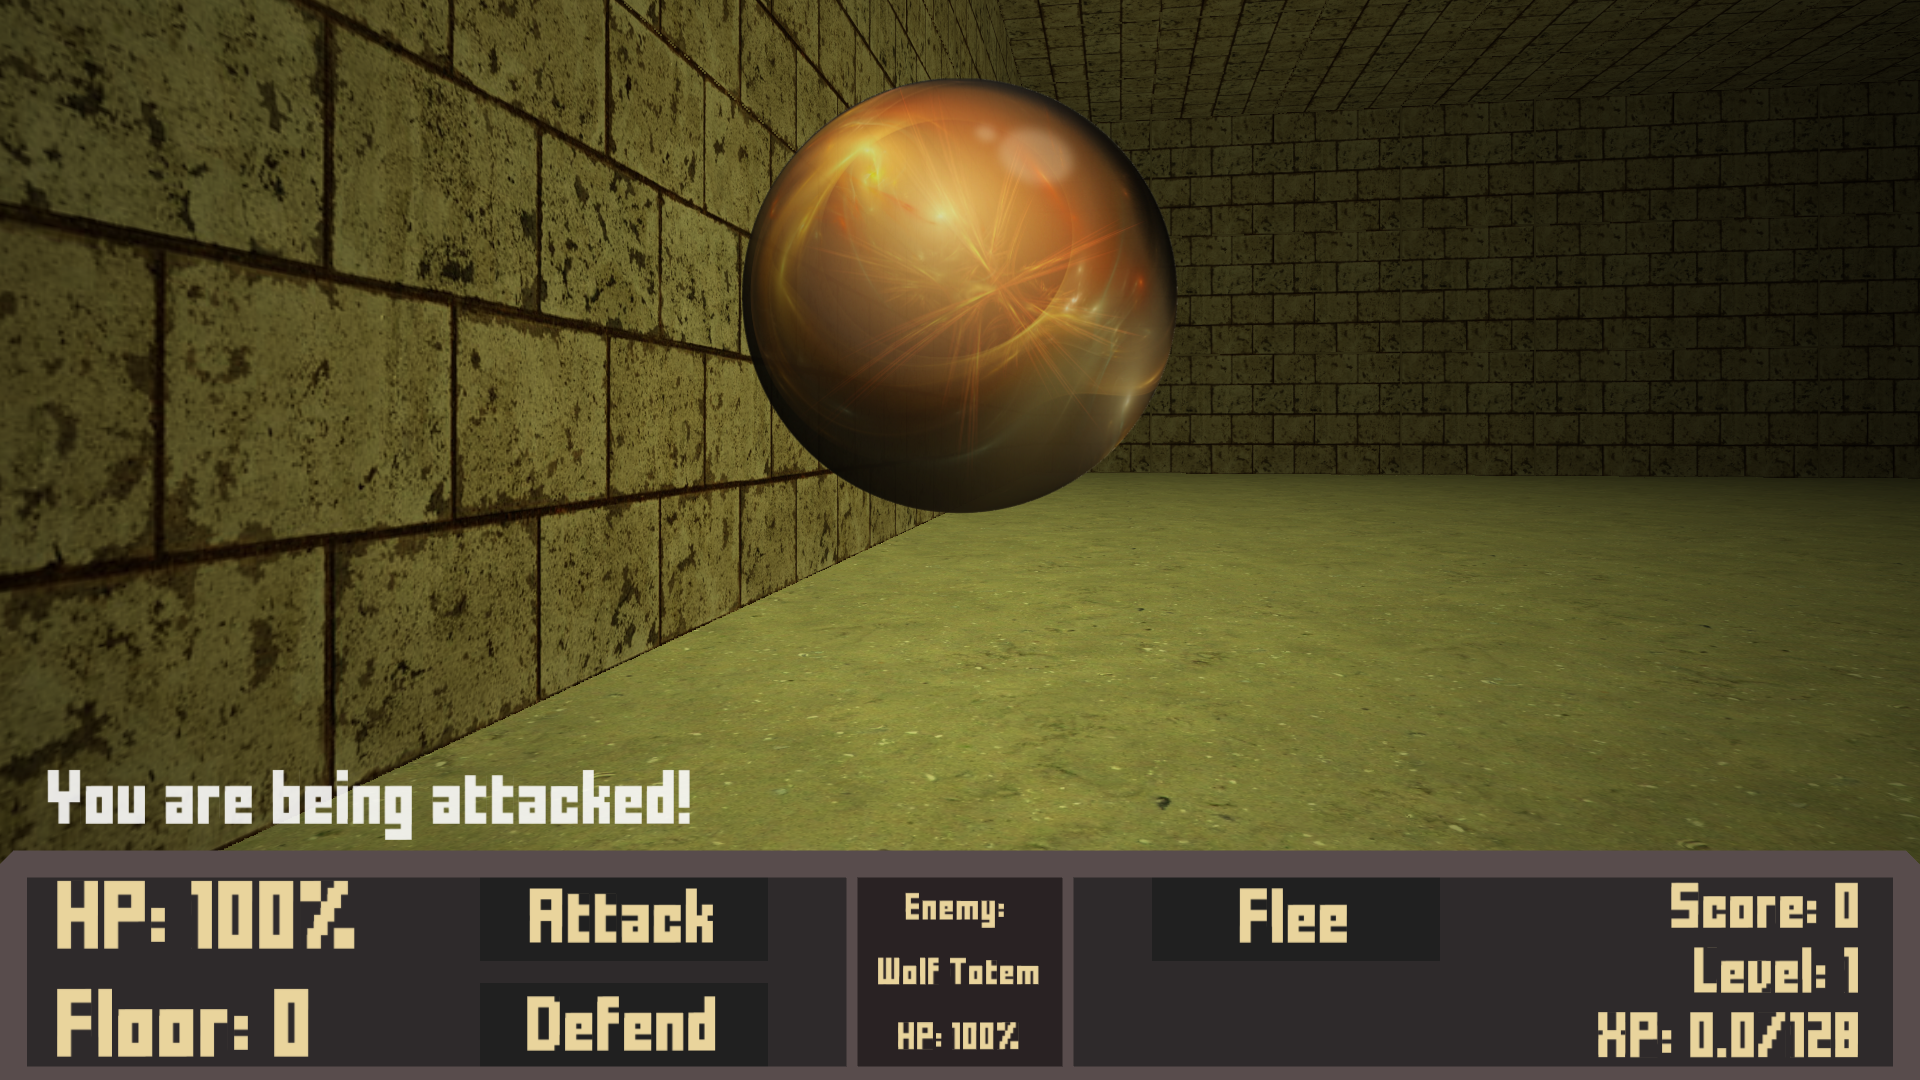
\includegraphics[width=.9\linewidth]{./versus-enemy.png}
\caption{Battle sequence}
\end{figure}


\section{Credits}
\label{sec:orgb159c77}
Thank you to the asset creators who made the sprites and textures for this game. They are cited below:

\begin{itemize}
\item \href{https://opengameart.org/content/496-pixel-art-icons-for-medievalfantasy-rpg}{Henrique lazarini} for his pixel art icons (Public Domain),
\item \href{https://opengameart.org/content/pietextureset}{Spiney} for his wall textures,
\item \href{https://opengameart.org/content/dirt-003}{Lamoot} for his dirt textures,
\item \href{https://www.deviantart.com/didier-bernard/art/sphere-PNG-version-300364281}{Didier Bernard} for his sphere sprite.
\end{itemize}
\end{document}
